138. \begin{figure}[ht!]
\center{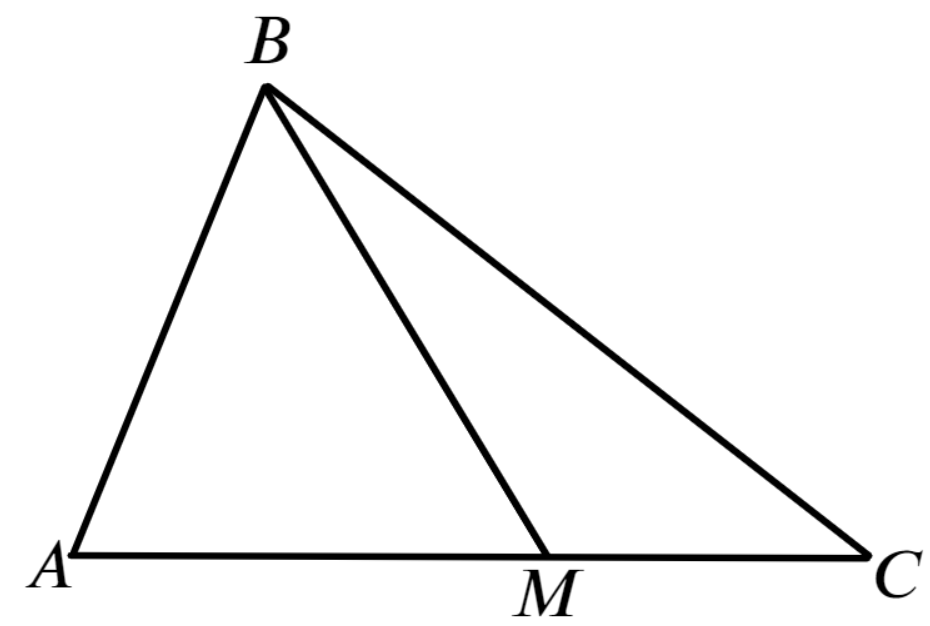
\includegraphics[scale=0.35]{g9-138.png}}
\end{figure}\\
Запишем теорему косинусов для треугольника $ABC:\ 9=36+25-2\cdot6\cdot5\cdot\cos(\angle A),$ откуда $\cos(\angle A)=\cfrac{13}{15}.$ Найдём $AM=\cfrac{3}{5}\cdot5=3$ и запишем теорему косинусов для треугольника $ABM:\ BM^2=36+9-2\cdot6\cdot3\cdot\cfrac{13}{15}=\cfrac{69}{5},$ значит $BM=\cfrac{\sqrt{345}}{5}.$\\
